\documentclass{article}
\usepackage{tikz,xstring}
\usetikzlibrary{shapes.geometric}

\begin{document}
\begin{centering}



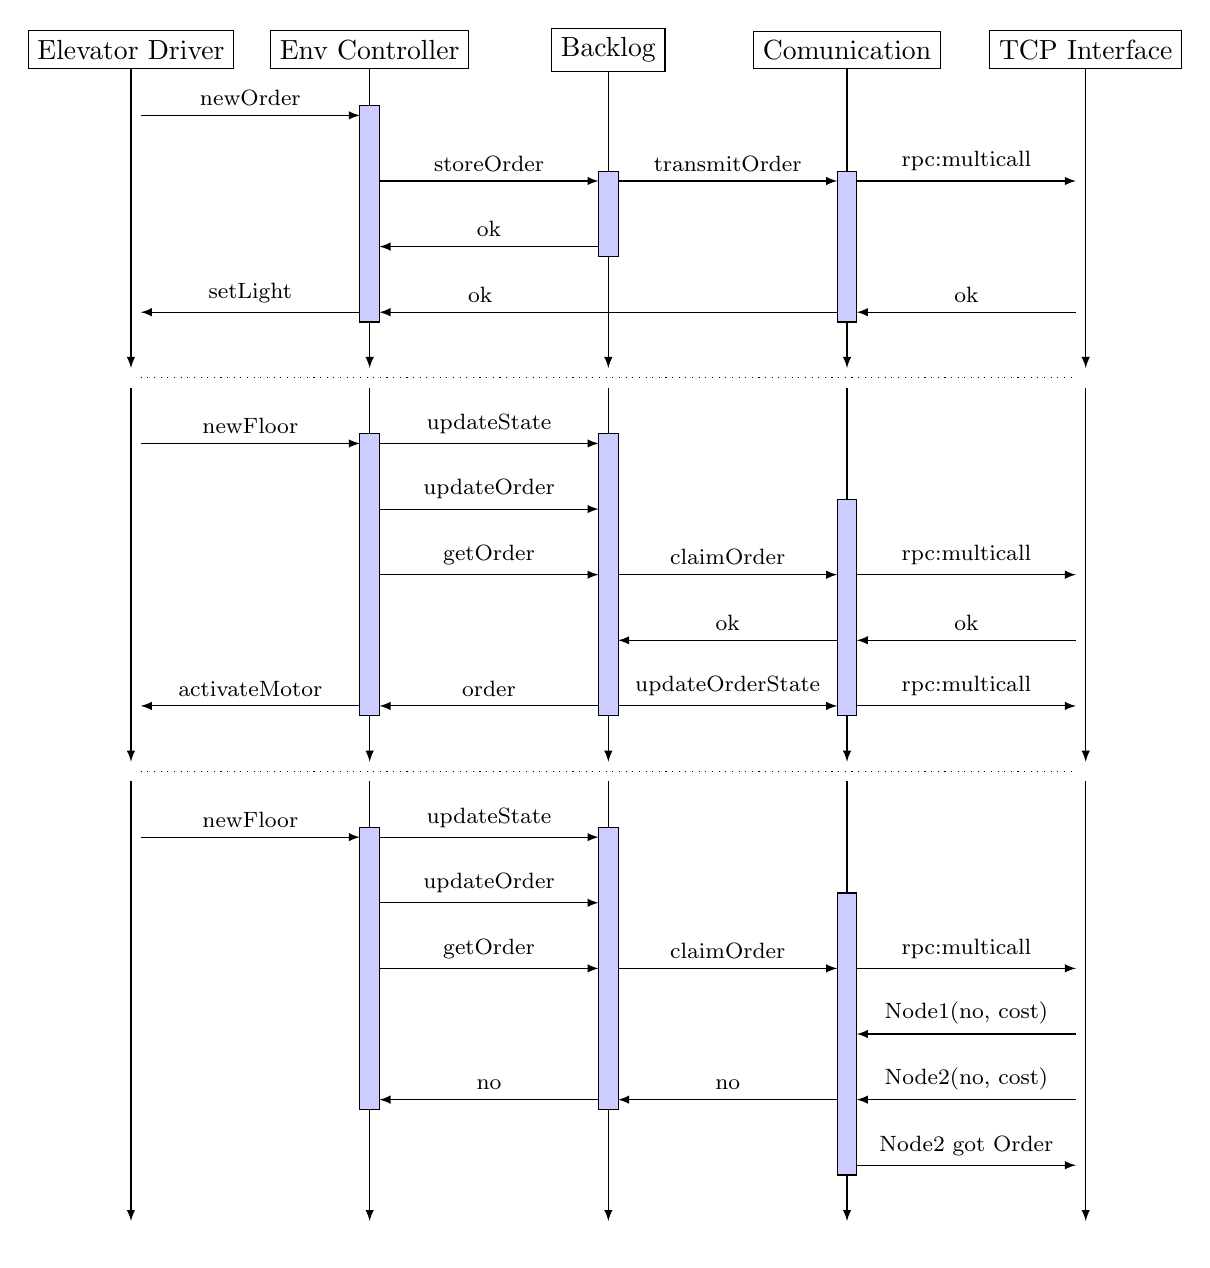
\begin{tikzpicture}

  \def\numberOfRows{18}
  % Agents
  \def\AgentList{Elevator Driver,Env Controller,Backlog,Comunication, TCP Interface}

  %determining the space betwen each point in the matrix
  \def\spaceRows{\textwidth/\numberOfColums} 
  \def\spaceColums{15/\numberOfRows}

  %Calculating stuff
  \StrCount{\AgentList}{,}[\arrlength]
  \def\numberOfColums{\arrlength}
  %Matrix
    \foreach \x in {0,...,\numberOfColums}
      \foreach \y in {0,...,\numberOfRows} 
         {\node(\x\y) at (\spaceRows*\x,-\spaceColums*\y) {};} %Label \x:\y when working, empty when done


  % Vertical lifelines
  \foreach \x in {0,...,\numberOfColums}
      {\draw [-latex] (\x0) -- (\x5);
      \draw [-latex] (\x5) -- (\x11);
      \draw [-latex] (\x11) -- (\x\numberOfRows);}

  %Agents labels
  \foreach \c [count=\x from 0] in \AgentList
      \fill (\x0) node[draw,fill=white] {\c};
      

  % Blocks 
  \filldraw[fill=blue!20]
     (11.north west) rectangle (14.south east)
     (22.north west) rectangle (23.south east)
     (32.north west) rectangle (34.south east);

  \filldraw[fill=blue!20]
     (16.north west) rectangle (110.south east)
     (26.north west) rectangle (210.south east)
     (37.north west) rectangle (310.south east);

  \filldraw[fill=blue!20]
     (112.north west) rectangle (116.south east)
     (212.north west) rectangle (216.south east)
     (313.north west) rectangle (317.south east);


  % Horizontal flows
  %Store Order
  \draw [-latex] (01) -- node[pos=0.5,font=\footnotesize, above] {newOrder} (11);
  \draw [-latex] (12) -- node[pos=0.5,font=\footnotesize, above] {storeOrder} (22);
  \draw [-latex] (22) -- node[pos=0.5,font=\footnotesize, above] {transmitOrder} (32);
  \draw [-latex] (32) -- node[pos=0.5,font=\footnotesize, above] {rpc:multicall} (42);
  \draw [-latex] (44) -- node[pos=0.5,font=\footnotesize, above] {ok} (34);
  \draw [-latex] (23) -- node[pos=0.5,font=\footnotesize, above] {ok} (13);
  \draw [-latex] (34) -- node[pos=0.78,font=\footnotesize, above] {ok} (14);
  \draw [-latex] (14) -- node[pos=0.5,font=\footnotesize, above] {setLight} (04);

  \draw [dotted]  (05) -- (45);
  %
  \draw [-latex] (06) -- node[pos=0.5,font=\footnotesize, above] {newFloor} (16);
  \draw [-latex] (16) -- node[pos=0.5,font=\footnotesize, above] {updateState} (26);
  \draw [-latex] (17) -- node[pos=0.5,font=\footnotesize, above] {updateOrder} (27);
  \draw [-latex] (18) -- node[pos=0.5,font=\footnotesize, above] {getOrder} (28);
  \draw [-latex] (28) -- node[pos=0.5,font=\footnotesize, above] {claimOrder} (38);
  \draw [-latex] (38) -- node[pos=0.5,font=\footnotesize, above] {rpc:multicall} (48);
  \draw [-latex] (49) -- node[pos=0.5,font=\footnotesize, above] {ok} (39);
  \draw [-latex] (39) -- node[pos=0.5,font=\footnotesize, above] {ok} (29);
  \draw [-latex] (210) -- node[pos=0.5,font=\footnotesize, above] {updateOrderState} (310);
  \draw [-latex] (310) -- node[pos=0.5,font=\footnotesize, above] {rpc:multicall} (410);
  \draw [-latex] (210) -- node[pos=0.5,font=\footnotesize, above] {order} (110);
  \draw [-latex] (110) -- node[pos=0.5,font=\footnotesize, above] {activateMotor} (010);

  \draw [dotted]  (011) -- (411);

  \draw [-latex] (012) -- node[pos=0.5,font=\footnotesize, above] {newFloor} (112);
  \draw [-latex] (112) -- node[pos=0.5,font=\footnotesize, above] {updateState} (212);
  \draw [-latex] (113) -- node[pos=0.5,font=\footnotesize, above] {updateOrder} (213);
  \draw [-latex] (114) -- node[pos=0.5,font=\footnotesize, above] {getOrder} (214);
  \draw [-latex] (214) -- node[pos=0.5,font=\footnotesize, above] {claimOrder} (314);
  \draw [-latex] (314) -- node[pos=0.5,font=\footnotesize, above] {rpc:multicall} (414);
  \draw [-latex] (415) -- node[pos=0.5,font=\footnotesize, above] {Node1(no, cost)} (315);
  \draw [-latex] (416) -- node[pos=0.5,font=\footnotesize, above] {Node2(no, cost)} (316);
  \draw [-latex] (316) -- node[pos=0.5,font=\footnotesize, above] {no} (216);
  \draw [-latex] (216) -- node[pos=0.5,font=\footnotesize, above] {no} (116);
  \draw [-latex] (317) -- node[pos=0.5,font=\footnotesize, above] {Node2 got Order} (417);



\end{tikzpicture}


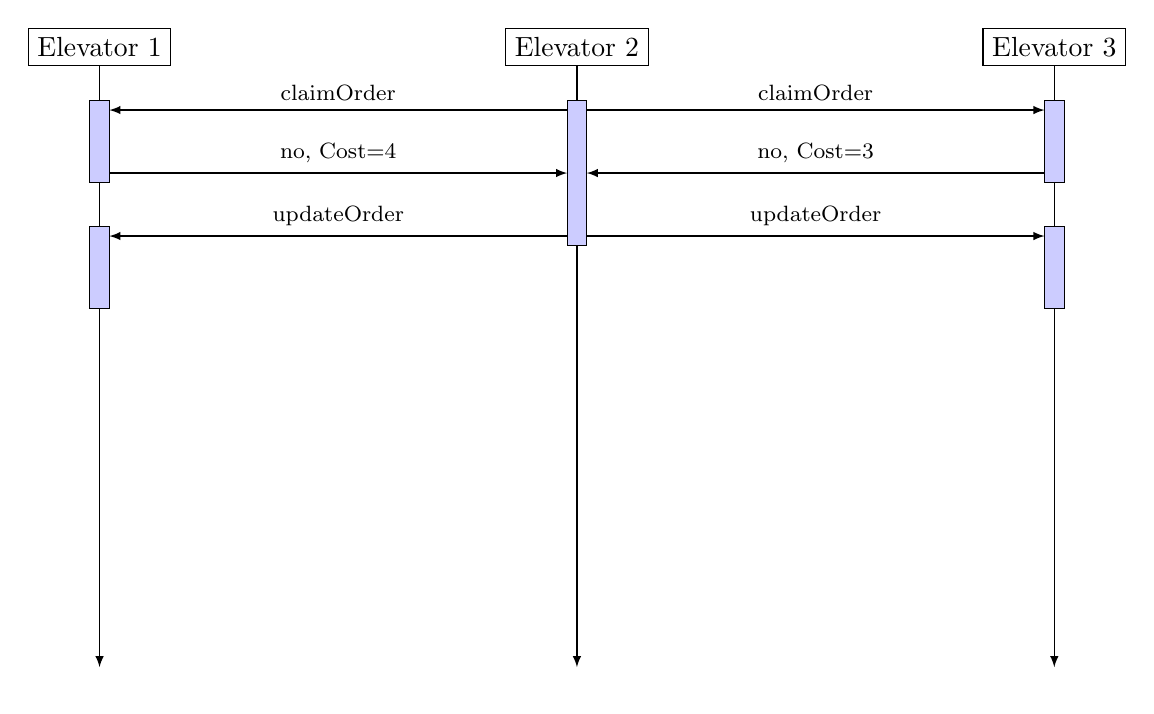
\begin{tikzpicture}

  \def\numberOfRows{10}
  % Agents
  \def\AgentList{Elevator 1, Elevator 2, Elevator 3}

  %determining the space betwen each point in the matrix
  \def\spaceRows{\textwidth/\numberOfColums} 
  \def\spaceColums{8/\numberOfRows}

  %Calculating stuff
  \StrCount{\AgentList}{,}[\arrlength]
  \def\numberOfColums{\arrlength}
  %Matrix
    \foreach \x in {0,...,\numberOfColums}
      \foreach \y in {0,...,\numberOfRows} 
         {\node(\x\y) at (\spaceRows*\x,-\spaceColums*\y) {};} %Label \x:\y when working, empty when done


  % Vertical lifelines
  \foreach \x in {0,...,\numberOfColums}
      {\draw [-latex] (\x0) -- (\x10);}

  %Agents labels
  \foreach \c [count=\x from 0] in \AgentList
      \fill (\x0) node[draw,fill=white] {\c};
      

 
  % Horizontal flows
  \draw [-latex] (11) -- node[pos=0.5,font=\footnotesize, above] {claimOrder} (21);
  \draw [-latex] (11) -- node[pos=0.5,font=\footnotesize, above] {claimOrder} (01);
  \draw [-latex] (02) -- node[pos=0.5,font=\footnotesize, above] {no, Cost=4} (12);
  \draw [-latex] (22) -- node[pos=0.5,font=\footnotesize, above] {no, Cost=3} (12);
  \draw [-latex] (13) -- node[pos=0.5,font=\footnotesize, above] {updateOrder} (23);
  \draw [-latex] (13) -- node[pos=0.5,font=\footnotesize, above] {updateOrder} (03);
  
   % Blocks 
  \filldraw[fill=blue!20] 
  (11.north west) rectangle (13.south east)
  (21.north west) rectangle (22.south east)
  (01.north west) rectangle (02.south east)
  (23.north west) rectangle (24.south east)
  (03.north west) rectangle (04.south east);



\end{tikzpicture}


\end{centering}
\end{document}  